\documentclass{article} % For LaTeX2e
\usepackage{nips14submit_e,times}
\usepackage{amsmath}
\usepackage{amsthm}
\usepackage{amssymb}
\usepackage{mathtools}
\usepackage{hyperref}
\usepackage{url}
\usepackage{algorithm}
\usepackage[noend]{algpseudocode}
%\documentstyle[nips14submit_09,times,art10]{article} % For LaTeX 2.09

\usepackage{graphicx}
\usepackage{caption}
\usepackage{subcaption}

\def\eQb#1\eQe{\begin{eqnarray*}#1\end{eqnarray*}}
\def\eQnb#1\eQne{\begin{eqnarray}#1\end{eqnarray}}
\providecommand{\e}[1]{\ensuremath{\times 10^{#1}}}
\providecommand{\pb}[0]{\pagebreak}
\DeclarePairedDelimiter\ceil{\lceil}{\rceil}
\DeclarePairedDelimiter\floor{\lfloor}{\rfloor}

\newcommand{\E}{\mathrm{E}}
\newcommand{\Var}{\mathrm{Var}}
\newcommand{\Cov}{\mathrm{Cov}}

\def\Qb#1\Qe{\begin{question}#1\end{question}}
\def\Sb#1\Se{\begin{solution}#1\end{solution}}

\newenvironment{claim}[1]{\par\noindent\underline{Claim:}\space#1}{}
\newtheoremstyle{quest}{\topsep}{\topsep}{}{}{\bfseries}{}{ }{\thmname{#1}\thmnote{ #3}.}
\theoremstyle{quest}
\newtheorem*{definition}{Definition}
\newtheorem*{theorem}{Theorem}
\newtheorem*{lemma}{Lemma}
\newtheorem*{question}{Question}
\newtheorem*{preposition}{Preposition}
\newtheorem*{exercise}{Exercise}
\newtheorem*{challengeproblem}{Challenge Problem}
\newtheorem*{solution}{Solution}
\newtheorem*{remark}{Remark}
\usepackage{verbatimbox}
\usepackage{listings}
\title{Probabilistic Method: \\
Problem Set V}


\author{
Youngduck Choi \\
CIMS \\
New York University\\
\texttt{yc1104@nyu.edu} \\
}


% The \author macro works with any number of authors. There are two commands
% used to separate the names and addresses of multiple authors: \And and \AND.
%
% Using \And between authors leaves it to \LaTeX{} to determine where to break
% the lines. Using \AND forces a linebreak at that point. So, if \LaTeX{}
% puts 3 of 4 authors names on the first line, and the last on the second
% line, try using \AND instead of \And before the third author name.

\newcommand{\fix}{\marginpar{FIX}}
\newcommand{\new}{\marginpar{NEW}}

\nipsfinalcopy % Uncomment for camera-ready version

\begin{document}


\maketitle

\begin{abstract}
This work contains solutions to the problem set V
of Probabilistic Method 2016 at Courant Institute of Mathematical Sciences.
\end{abstract}

\bigskip

\begin{question}[1]
\hfill
\begin{figure}[h!]
  \centering
    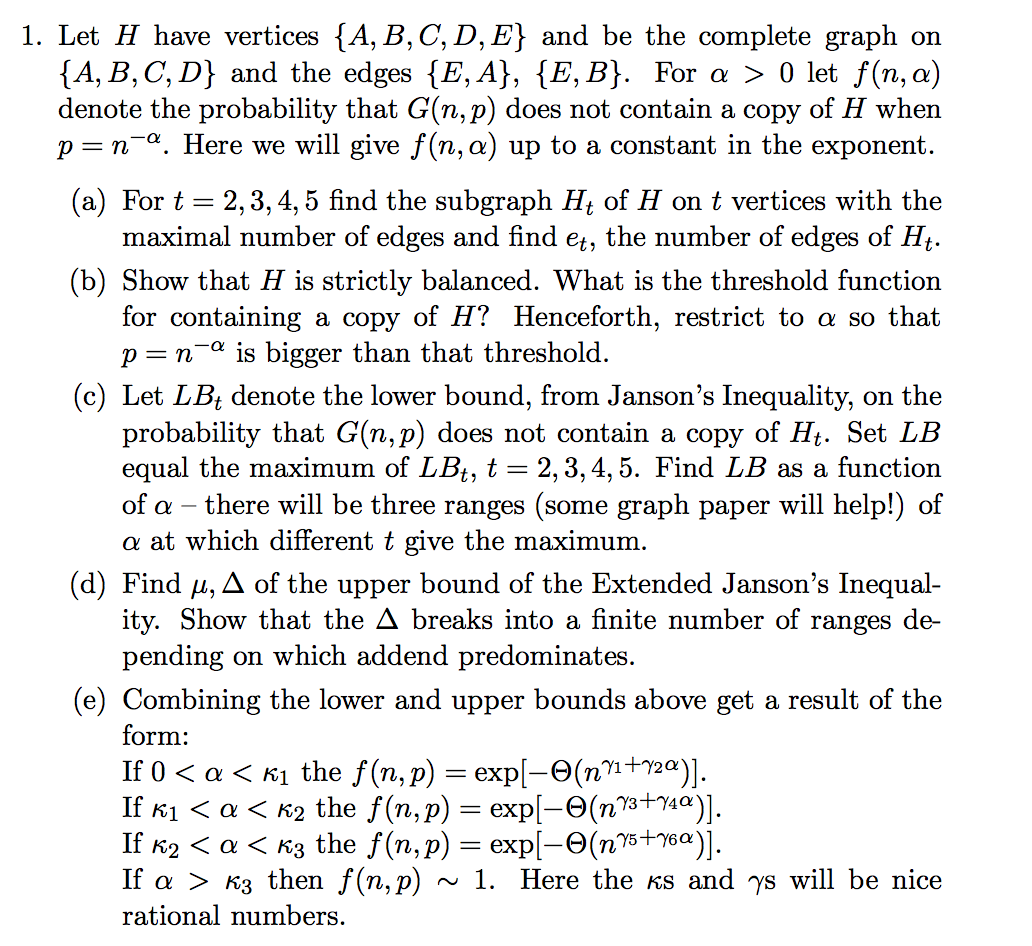
\includegraphics[width=0.7\textwidth]{pm-5-1.png}
\end{figure}
\end{question}
\newpage
\begin{solution} \hfill \\
\textbf{(a)} We have $e_2 = 1$, $e_3 = 3$, $e_4 = 6$, and $e_5 = 8$.  

\bigskip

\textbf{(b)} $n^{-\frac{5}{8}}$ is the threshold function as $\dfrac{1}{2}, 1, \dfrac{6}{4}$ 
is less than $\dfrac{8}{5}$, which also reveals that $H$ is strictly balanced.

\bigskip

\textbf{(c)} We have
\eQb
P(\text{ G has no } K_i) \leq (1-p^{f_i})^{{n \choose i}} \sim \exp(-\Theta(n^i - f_i \alpha )),  
\eQe
where $f_i = 1,3,6,8$. 

\bigskip

\textbf{(d)}

\bigskip

\textbf{(e)} 

\end{solution}

\newpage

\begin{question}[2]
\hfill
\begin{figure}[h!]
  \centering
    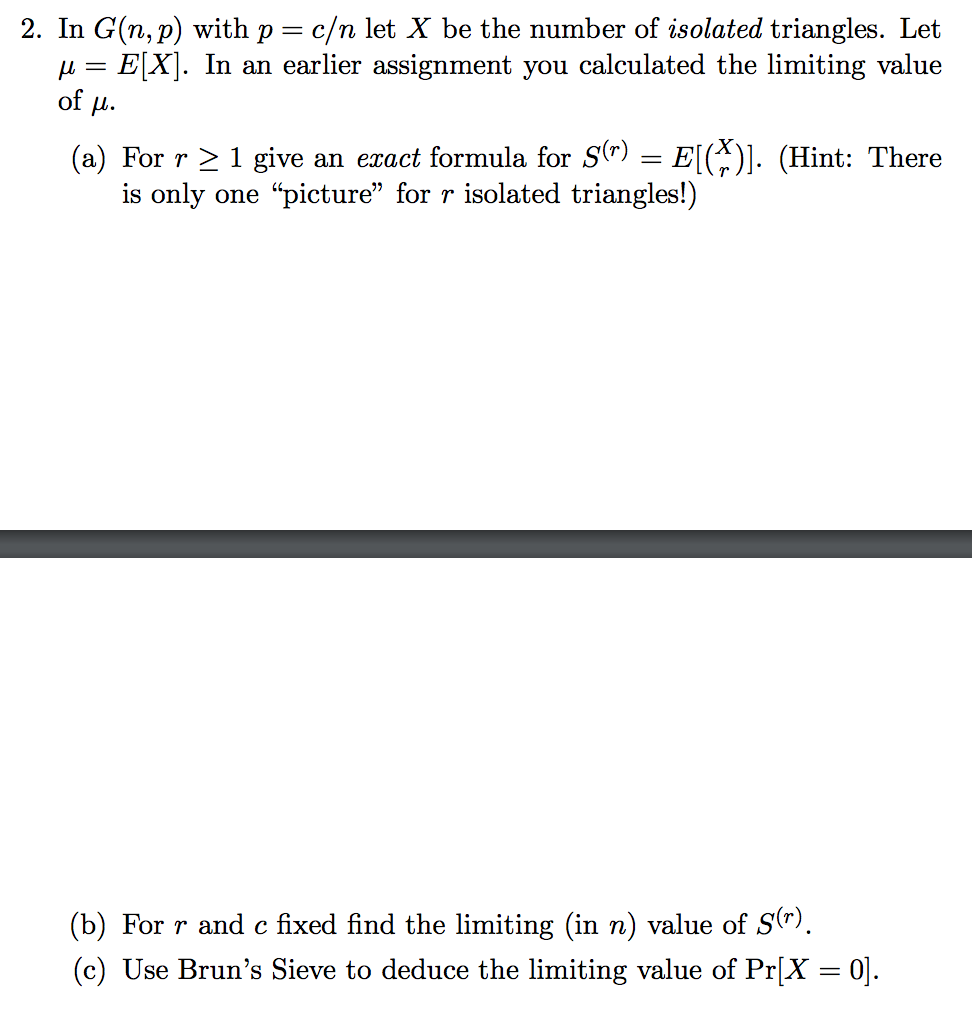
\includegraphics[width=0.8\textwidth]{pm-5-2.png}
\end{figure}
\end{question}
\begin{solution}
\textbf{(a)}
By counting, we know that there are $\dfrac{1}{r!}\prod_{i=0}^{r-1}{ n-3 
\choose 3}$ cases of isolated triangles. Hence, we have the exact formula as
\eQb
E{X \choose r}] &=& \dfrac{1}{r!} \prod_{i=0}^{r-1} {n -3i \choose 3} (1-p)^{3r(n-3r)+9{r \choose 2}}.
\eQe

\bigskip

\textbf{(b)} As $(1-p)^{3r(n-3r)+9{r \choose 2}} \sim (1-p)^{r(3n-9)}$, we have
\eQb
E[X] \sim \dfrac{u^r}{r!}.
\eQe 

\bigskip

\textbf{(c)} By Brun's Sieve, we have that the limiting value of $P(X = 0)$ is
$e^{\frac{c^3e^{-3c}}{6}}$.
 
\hfill $\qed$

\end{solution}

\newpage

\begin{question}[3]
\hfill
\begin{figure}[h!]
  \centering
    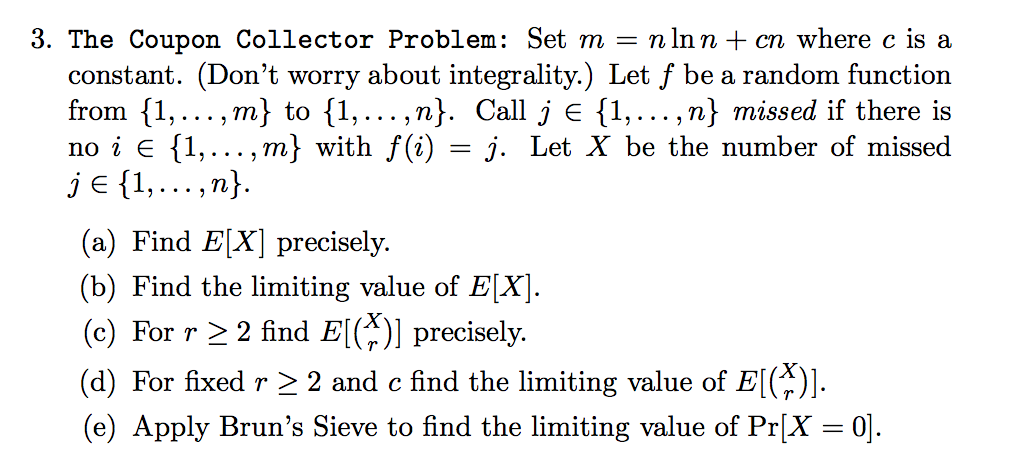
\includegraphics[width=0.8\textwidth]{pm-5-3.png}
\end{figure}
\end{question}
\begin{solution}
\textbf{(a)}
For, $1 \leq i \leq n$, let $B_i$ denote the event, where $i$ is missed, and $X_i$ be the indicator
random variable for $B_i$. Let $X = \sum_{i=1}^{n} X_i$. By Linearity of Expectation, it follows that
\eQb
E[X] &=& E[\sum_{i=1}^{n} X_i] = \sum_{i=1}^{n} E[X_i] = \sum_{i=1}^{n} P(B_i) \\ 
&=& n(\dfrac{n-1}{n})^m = n(\dfrac{n-1}{n})^{n\ln(n) + cn}.
\eQe 

\bigskip

\textbf{(b)} 
With an argument involving Taylor series, which was used in class previously, we know that 
$n(1-\dfrac{1}{n})^{m} ~ ne^{-\frac{m}{n}}$. Hence, it follows that $E[X] \sim e^{-c}$.

\bigskip

\textbf{(c)} By counting, we have
\eQb
E[{X \choose r}] &=& {n \choose r}(1-\dfrac{r}{n})^{m}.
\eQe

\bigskip

\textbf{(d)} Similar to $(b)$, we have
\eQb
E[{X \choose r}] &\sim&\dfrac{1}{r!}(ne^{-\frac{m}{n}})^{r} \sim \dfrac{\mu^r}{r!}. 
\eQe

\bigskip

\textbf{(e)} By Brun's Sieve, we have $P(X = 0) \to e^{-e^{-c}}$.

\hfill $\qed$
\end{solution}

\newpage

\begin{question}[4]
\hfill
\begin{figure}[h!]
  \centering
    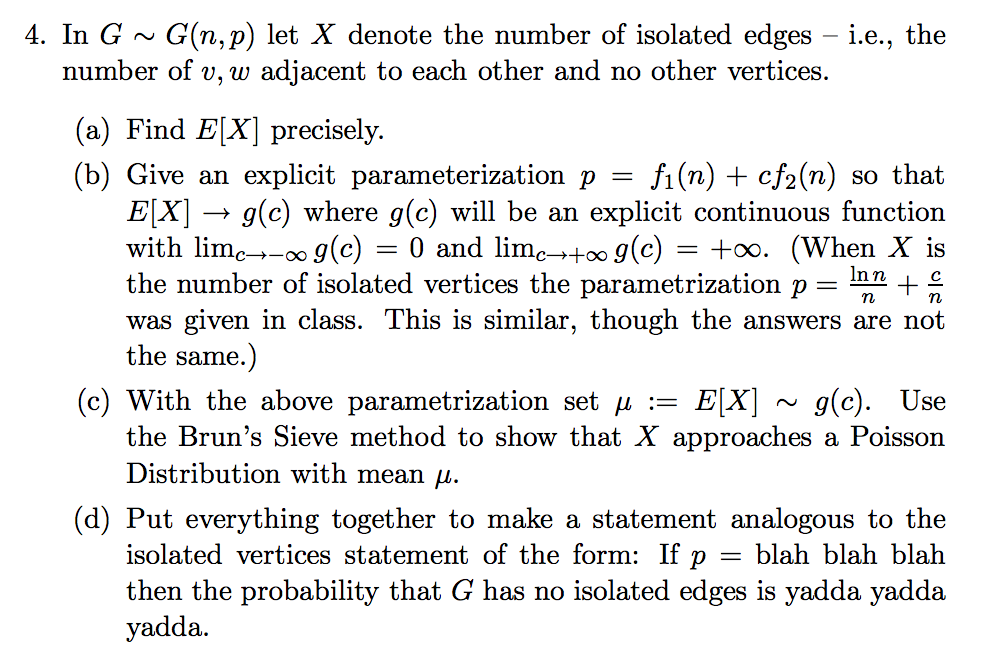
\includegraphics[width=1\textwidth]{pm-5-4.png}
\end{figure}
\end{question}
\begin{solution}
\textbf{(a)} Let $B_i$ denote the event, where $i$th edge from the index set of edges $I$, is
an isolated edge for $i = 1,2...,{n \choose 2}$. Let $X_i$ be the indicator random variable for $B_i$,
and $X = \sum_{i \in I} X_i$. By linearity of expectation, it follows that
\eQb
E[X] &=& \sum_{i \in I} E[X_i] = {n \choose 2} p(1-p)^{2(n-2)},
\eQe  
as $E[X_i] = P(X_i) = p(1-p)^{2(n-2)}$ with $2(n-2)$ edges required not to be present. 

\bigskip

\textbf{(b)}
Consider the following parametrization:
\eQb
p &=& \dfrac{\ln(n)}{2n} + \dfrac{\ln(\ln(n)}{2n} + \dfrac{c}{n}. 
\eQe
Then, it follows that
\eQb
E[X] \sim \dfrac{n^2}{2}{\ln(n)}{2n} e^{-\ln(n) - \ln(\ln(n)- c} = \dfrac{e^{-c}}{4}.
\eQe
\bigskip

\textbf{(c)} By counting, we have
\eQb
E[{n \choose r}] &=& \dfrac{1}{r!}\prod_{i=0}^{r-1} {n-2i \choose 2} 
p^r(1-p)^{2r(n-2)-2r(n-1)} \\
&\sim& {n \choose 2}^r \dfrac{1}{r!}(p(1-p)^{2(n-2)})^r \sim \dfrac{\mu^r}{r!} \\
\eQe
$S^{(r)} \sim \dfrac{u^r}{r!}$. Hence, $X$ approaches Poisson in the limit.

\bigskip

\textbf{(d)}
If $p = \dfrac{\ln(n)}{2n} + \dfrac{\ln(\ln(n)}{2n} + \dfrac{c}{n}$, then the probability
that G has no isolated edges is $e^{\frac{-e^{-c}}{4}} + o(1)$.  
 
\hfill $\qed$
\end{solution}

\end{document}

